\section{Explainability with SHAP}
\label{sec:shap}

\paragraph{Method.} SHAP splits one prediction into a reference value plus one
contribution per feature: $f(x) = \phi_0 + \sum_j \phi_j(x)$, where $\phi_0$ is
the base value. For LightGBM, \code{TreeExplainer} computes these values
exactly, in log-odds of \pos: a positive value pushes the prediction towards
\pos. We explain the final model on 1{,}000 people drawn from the development
set; the test set stays untouched. One-hot encoding splits each categorical
feature into several columns, and SHAP values are additive, so we sum the
values of the columns of each original feature (e.g.\ all the
\code{relationship} columns) to get one contribution per feature. As a check,
for every explained person, the base value plus the sum of the contributions
gives back the raw score, and its sigmoid gives back the predicted probability.

\paragraph{Global importance.} The global importance of a feature is its mean
absolute SHAP value over the 1{,}000 people: how much it moves the
predictions on average, whatever the direction. The beeswarm plot adds the
direction (Figure~\ref{fig:shap-global}). Marital status comes first by far
(mean $|\text{SHAP}|$ of 0.93 in log-odds), followed by age (0.58), capital
gains (0.53), relationship (0.41) and our interaction
\code{education\_x\_hours} (0.39); occupation (0.31) and \code{education-num}
(0.30) come next. Sex is 9th (0.18) and race 14th (0.06) out of 15.

The beeswarm, drawn per encoded column before the sum, shows the direction of
each effect. Being married to a civilian spouse pushes the score up by about
$+0.8$, and not being married pulls it down by about as much. Young ages pull it
down strongly (to about $-2.5$), while middle and older ages push it up. Most
people have no capital gain, which pulls the score down slightly, but a large
gain pushes it up by $+4$ to $+7$: the largest single effects of the model.
Higher education and more \code{education\_x\_hours} push the score up.

\begin{figure}[H]
\centering
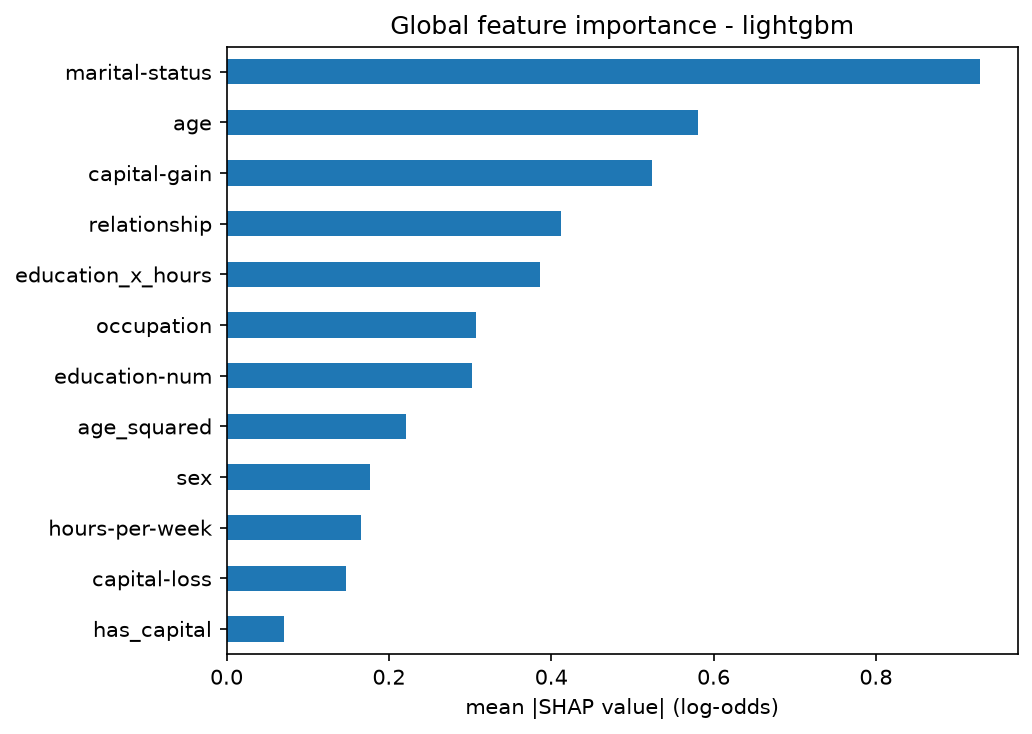
\includegraphics[width=0.48\textwidth]{shap_global_importance.png}\hfill
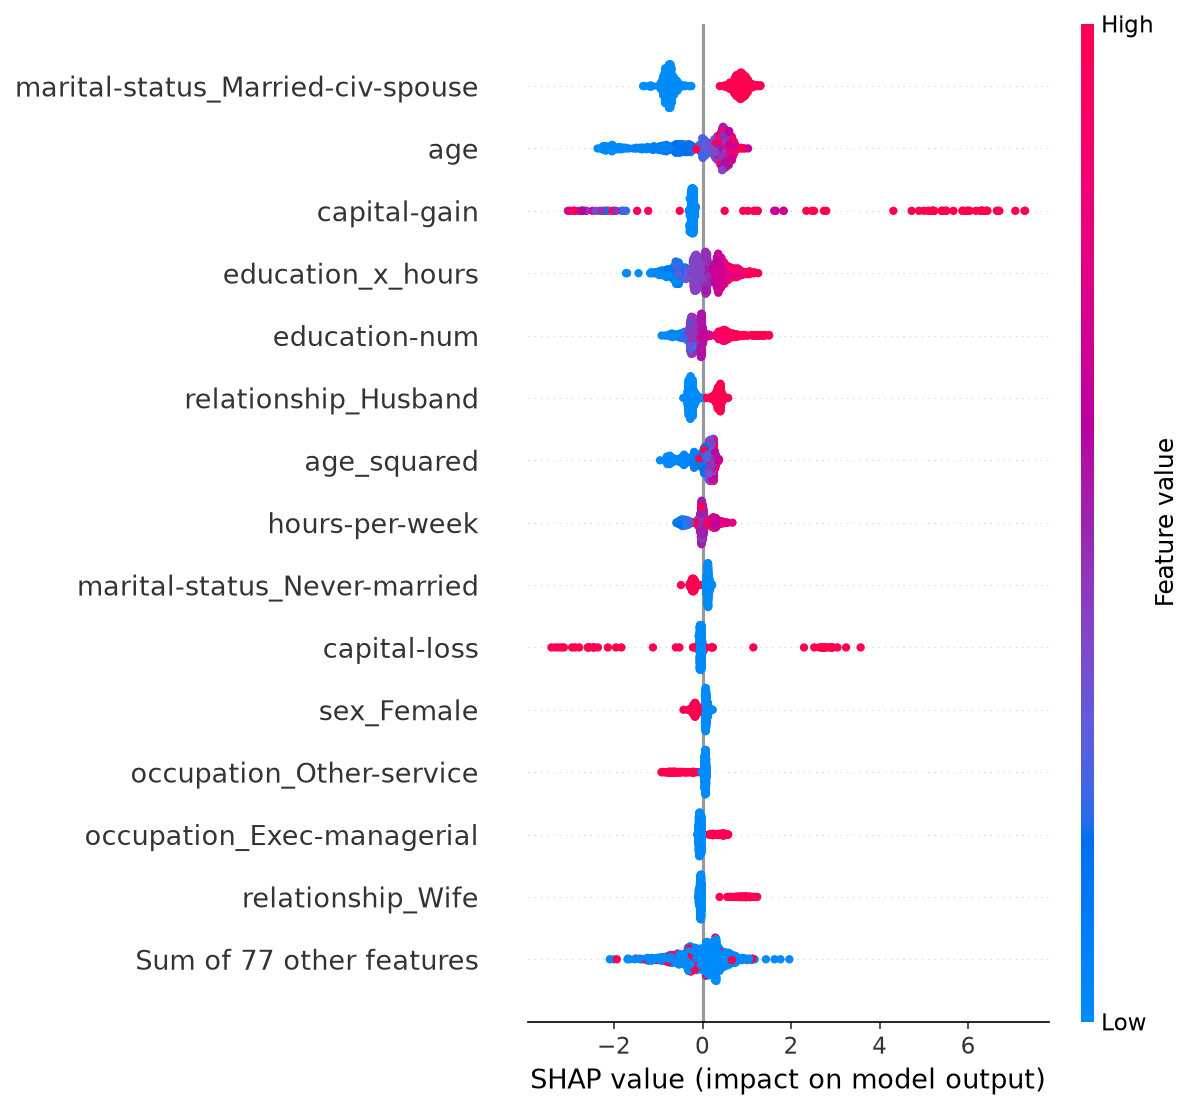
\includegraphics[width=0.48\textwidth]{shap_beeswarm.png}
\caption{Global SHAP importance per original feature (left) and beeswarm plot
per encoded column (right) of the final model, on 1{,}000 people of the
development set.}
\label{fig:shap-global}
\end{figure}

\paragraph{Local explanations.} We explain three people: the most confident
\pos{} prediction, the most confident \negc{} prediction, and the person
closest to the decision threshold (Figure~\ref{fig:shap-local}). All three
start from the base value $\phi_0 = -1.93$ (a probability of 0.13).
\begin{itemize}
  \item \textbf{Most confident \pos{}} ($P = 0.999$, truly \pos). A capital
  gain of \$15{,}024 adds $+5.67$ on its own, more than half of the total
  push of $+9.26$. Being married ($+0.74$), 16 years of education ($+0.61$),
  their product with 50 hours a week ($+0.50$) and an executive job ($+0.39$)
  add the rest.
  \item \textbf{Most confident \negc{}} ($P < 0.001$, truly \negc). Age 18 is
  the main reason: $-2.17$ for \code{age} and $-0.79$ for
  \code{age\_squared}. Little education times few hours ($-1.18$), never
  married ($-0.90$) and a farming job ($-0.50$) push in the same direction.
  \item \textbf{Closest to the threshold} ($P = 0.539$, just below the
  threshold of 0.54, so predicted \negc; truly \negc). A married man of 35
  with a high \code{education\_x\_hours}: being married ($+0.88$), the
  interaction ($+0.63$) and being a husband ($+0.36$) push up, but the absence
  of capital gains ($-0.21$) keeps him just under the threshold.
\end{itemize}

\begin{figure}[H]
\centering
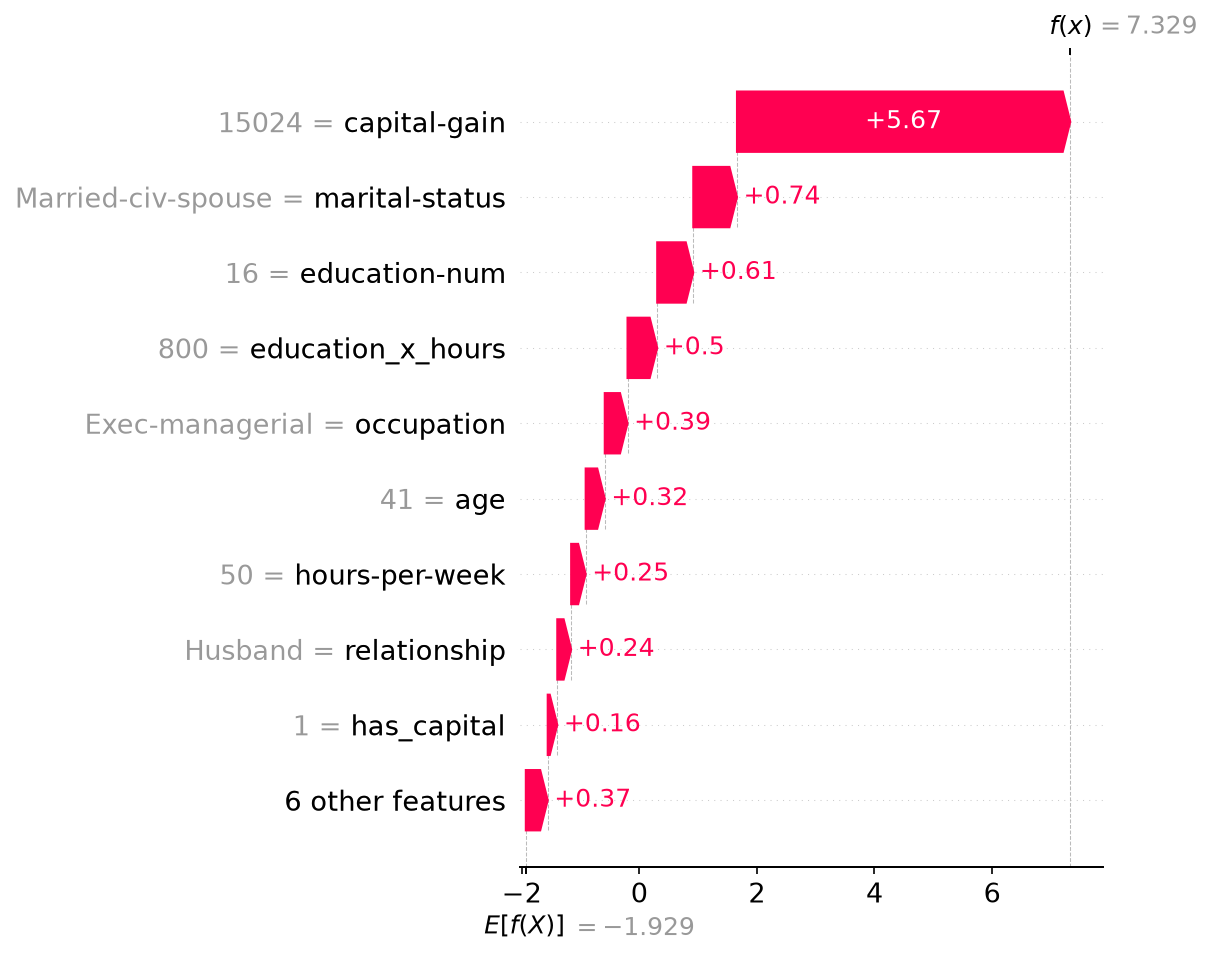
\includegraphics[width=0.48\textwidth]{shap_local_most_likely_above_50k.png}\hfill
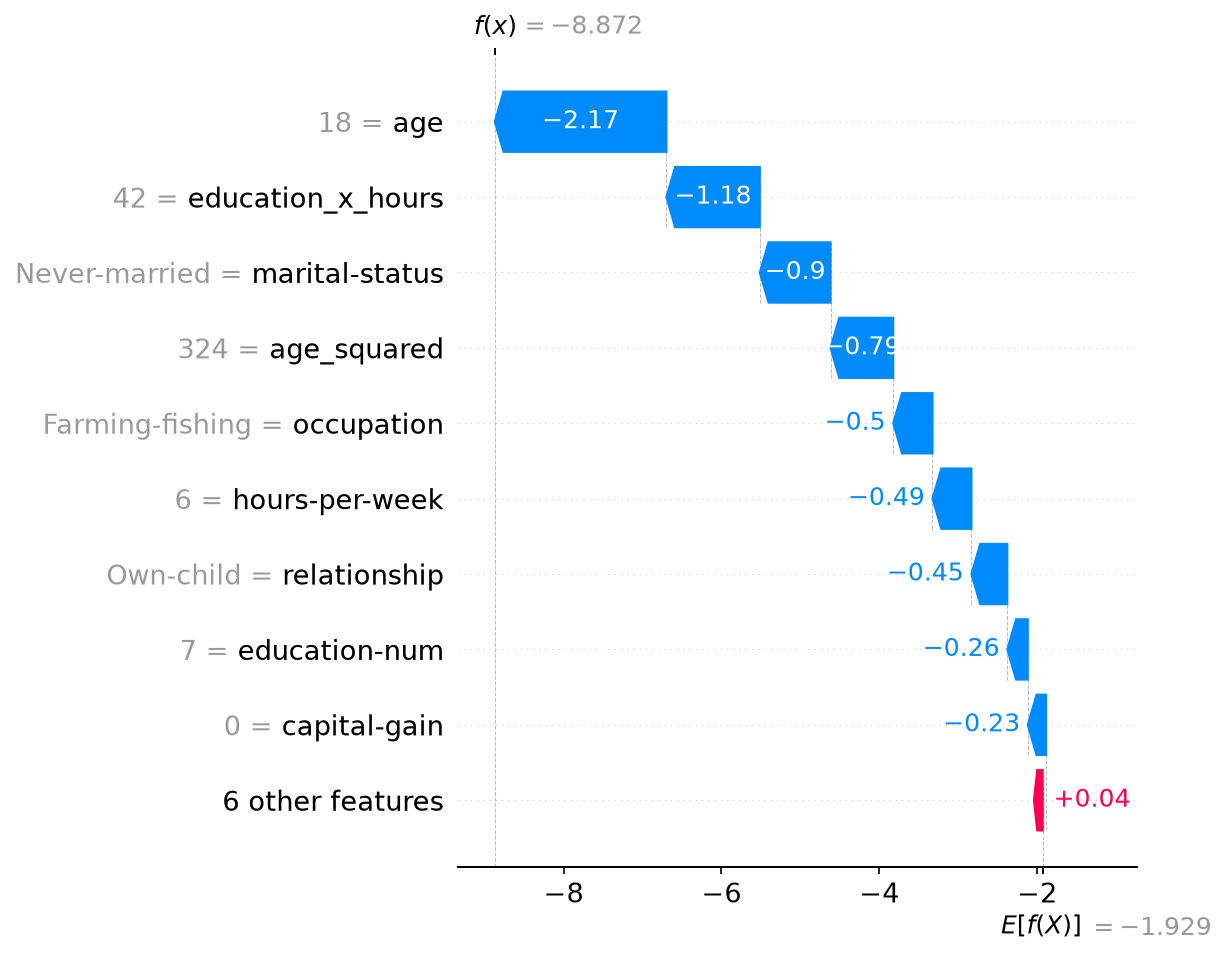
\includegraphics[width=0.48\textwidth]{shap_local_least_likely_above_50k.png}\\[4pt]
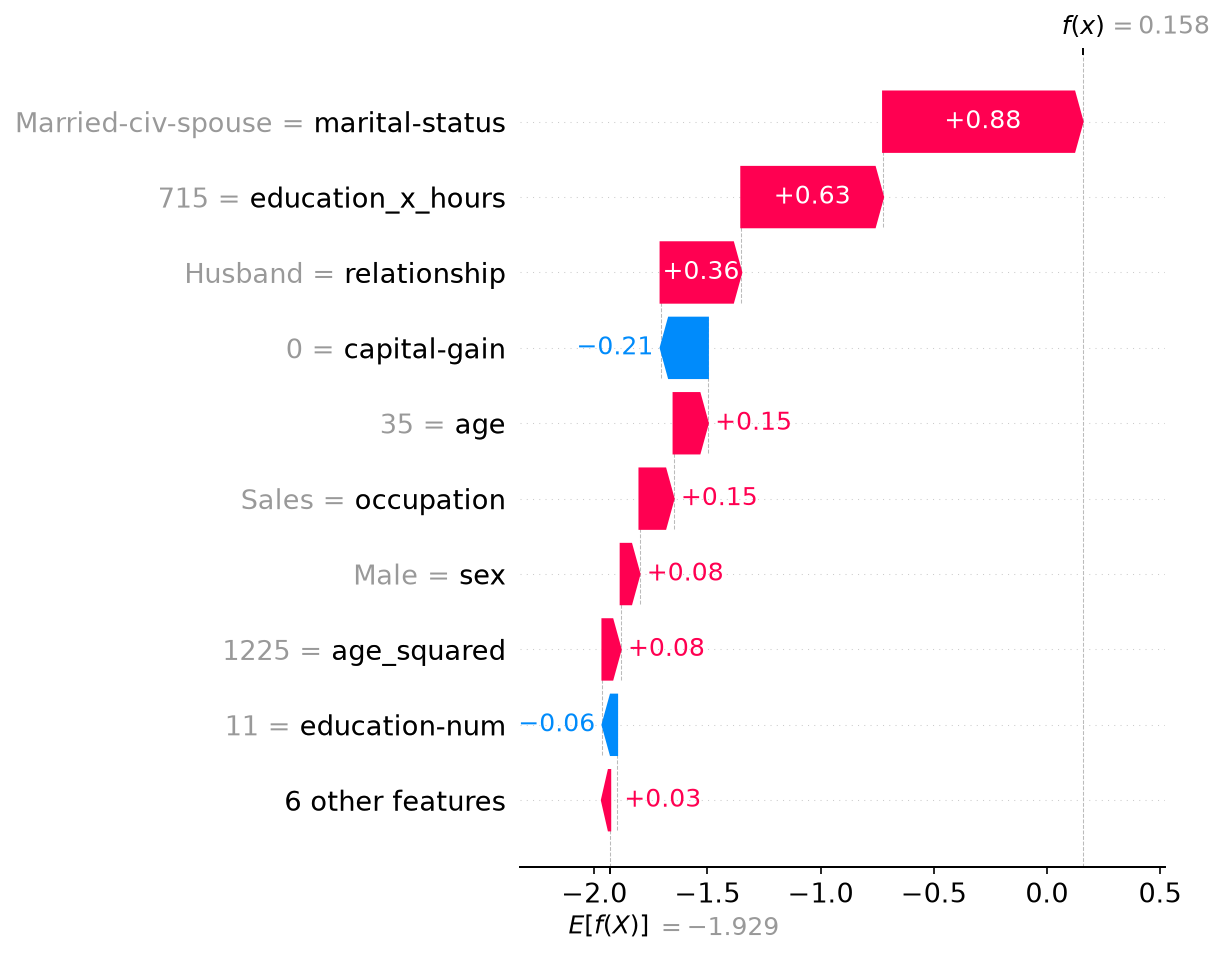
\includegraphics[width=0.48\textwidth]{shap_local_borderline.png}
\caption{Waterfall plots of the most confident \pos{} (top left), the most
confident \negc{} (top right) and the person closest to the threshold
(bottom): from the base value, each feature pushes the score up (red) or down
(blue) until the final prediction.}
\label{fig:shap-local}
\end{figure}

\paragraph{Do the important features make business sense?} Mostly yes. The
household variables come first (marital status and relationship together weigh
1.34): being married is a proxy for age, career stage and a stable household.
Capital gains are a direct sign of wealth, and age, education and occupation
describe a career. These are the drivers one would expect for income. Our
engineered features are used (Section~\ref{sec:features}):
\code{education\_x\_hours} is 5th, ahead of \code{education-num} itself, and
\code{age\_squared} is 8th; \code{has\_capital} is only 12th, because the trees
can split on \code{capital-gain} directly. Sex (9th) and race (14th) weigh
less, but not zero: being a woman lowers the score by about $0.3$ in log-odds
in the beeswarm, on top of what passes through \code{relationship}
(\code{Husband} / \code{Wife}). The model reproduces the income gap between
men and women in the 1994 census; with the fairness audit out of scope, we
flag it as a limitation rather than measure it. Two cautions apply to this
reading. SHAP explains what the model
does, not what causes a high income: being married does not raise anyone's
income in itself. And correlated features share the credit: \code{age} and
\code{age\_squared}, \code{marital-status} and \code{relationship}, or
\code{education-num} and \code{education\_x\_hours} must be read together.
